\begin{align}
    P(v) &\sim \frac{v^2}{K_B T} \exp \left( - \frac{m v^2}{2K_B T} \right)  \\ 
    P(v_x) &\sim \frac{1}{\sqrt{K_B T}}\exp \left( - \frac{m v_x^2}{2K_B T} \right)\\
    P(v_y) &\sim \frac{1}{\sqrt{K_B T}}\exp \left( - \frac{m v_y^2}{2K_B T} \right)
\end{align}





\begin{figure}[h!]
    \centering
    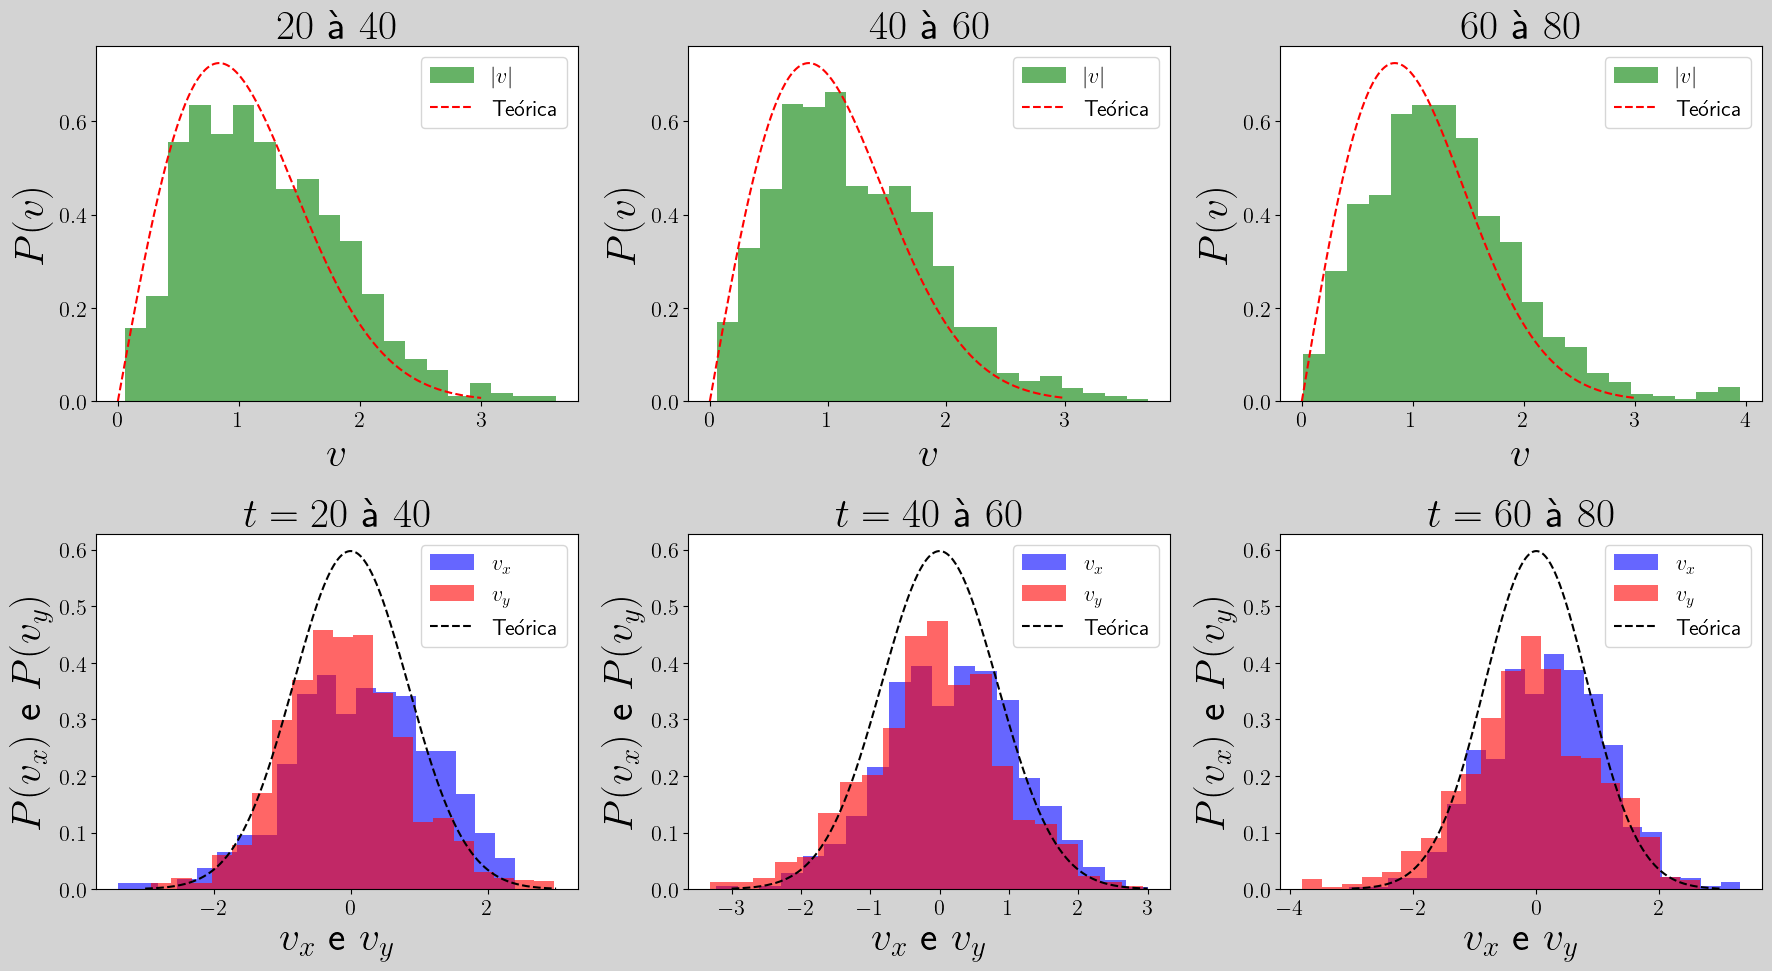
\includegraphics[width=0.7\linewidth]{tarefa-B/distribuicoes-b.png}
    \caption{Distribuição da velocidade, magnitude e componentes em intervalos $t=20-40$, $t=40-60$ e $t=60-80$.}
    \label{fig:distribuicoes-velocidade-b}
\end{figure}


Além disso há um gif para essa simulação.

\clearpage